

%%%%% MOTIVATION & INTRODUCTION
\frame{
\begin{tikzpicture}[remember picture,overlay]
\fill[blue1]
(current page.north west) rectangle ([xshift=0.55\paperwidth,yshift=0.27\paperheight]current page.west|-{pic cs:end});
\end{tikzpicture}
\begin{textblock}{0.55}(0.02,0.03)
	\textcolor{white}{							
	\Large{X-ray radiography of granular systems \\
		-- particle densities and dynamics}
	}
\end{textblock}

\begin{textblock}{0.15}(0.05,0.2)
\includegraphics[width=\textwidth]{Sources/motivation/sand.png}
\\[0.2cm]
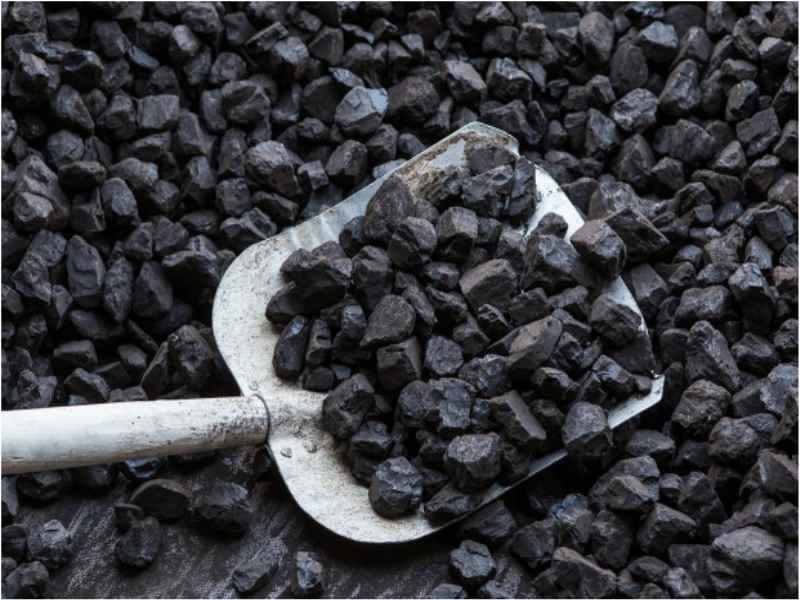
\includegraphics[width=\textwidth]{Sources/motivation/coal.png}
\\[0.2cm]
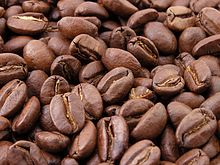
\includegraphics[width=\textwidth]{Sources/motivation/coffee.png}
{\Huge$\vdots$}
\end{textblock}

\begin{textblock}{0.35}(0.25,0.2)
\visible<2->{
\centering
\textbf{Granular materials are athermal}\\[0.1cm]
\begin{minipage}[c]{0.25\textwidth}
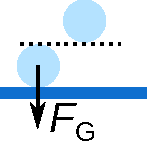
\includegraphics[width=\textwidth]{Sources/motivation/lift_particle.pdf}
\end{minipage}
\hfill
\begin{minipage}[c]{0.6\textwidth}
\begin{align}
E_\text{pot} &\approx \textcolor{red}{10^{10}} E_\text{thermal}\nonumber
\end{align}
\end{minipage}
}
\end{textblock}

\begin{textblock}{0.35}(0.25,0.5)
\centering
\visible<4->{
\textbf{Dissipative interactions}\\[0.1cm]
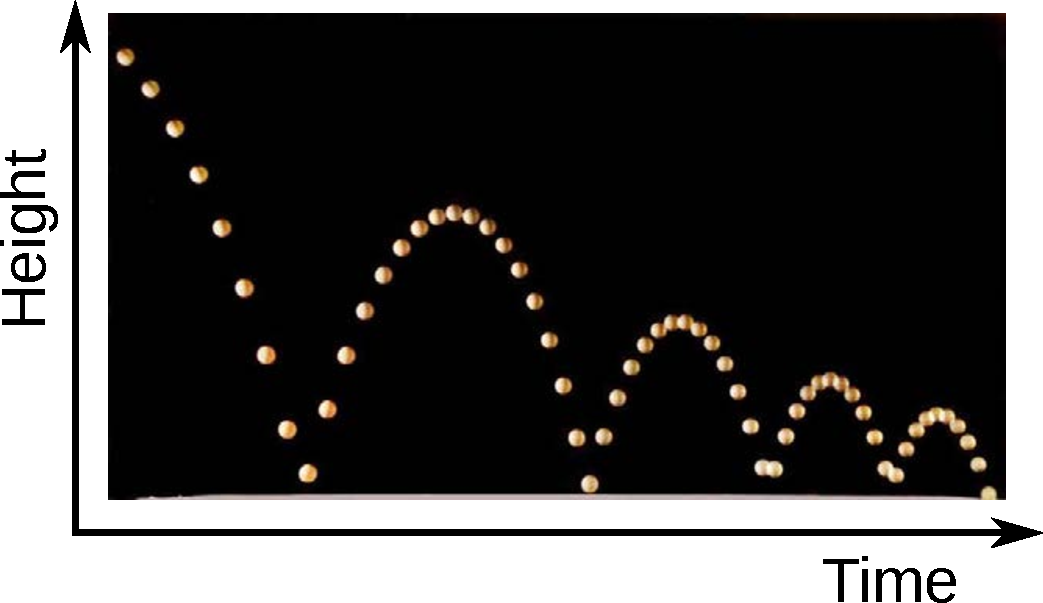
\includegraphics[width=\textwidth]{Sources/motivation/Driscoll_et_al_2016.pdf}\\
{\scriptsize Driscoll \textit{et al} (2016)}}
\end{textblock}

\begin{textblock}{0.25}(0.7,0.1)
\centering
\visible<3->{
\textbf{Volume fraction} 
\[\Phi = \frac{V_\text{Particles}}{V_\text{Container}}\]}
\only<3>{
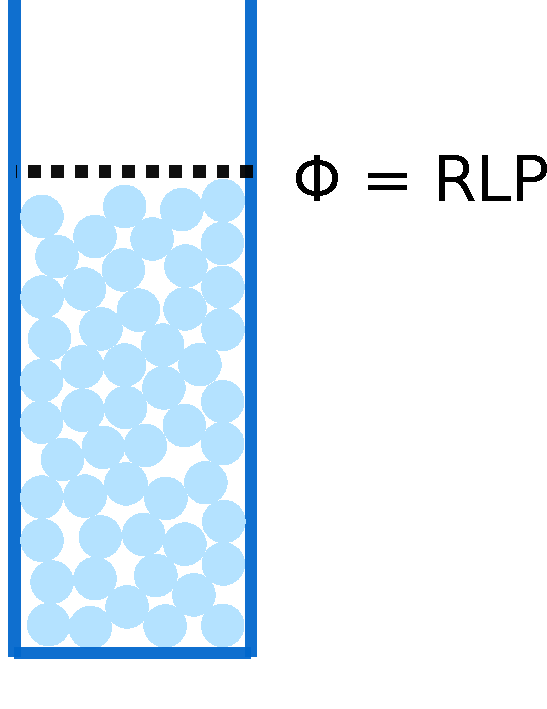
\includegraphics[width=\textwidth]{Sources/motivation/setup-fluidized_bed_sedimented.pdf}}
\only<4>{
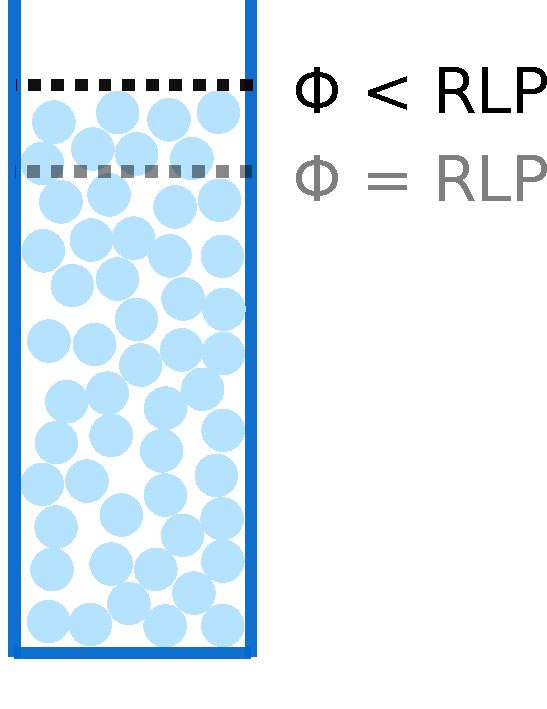
\includegraphics[width=\textwidth]{Sources/motivation/setup-fluidized_bed_expanded.pdf}}
\end{textblock}
}



%%%%% Motivation fluidized bed
\frame{
\begin{tikzpicture}[remember picture,overlay]
\fill[blue1]
(current page.north west) rectangle ([xshift=0.55\paperwidth,yshift=0.27\paperheight]current page.west|-{pic cs:end});
\end{tikzpicture}
\begin{textblock}{0.55}(0.02,0.03)
	\textcolor{white}{							
		\Large{X-ray radiography of granular systems \\
			-- particle densities and dynamics}
	}
\end{textblock}
	
\begin{textblock}{0.55}(0.02,0.2)
\visible<1->{
	\textbf{Liquid fluidized bed}\\[0.5cm]
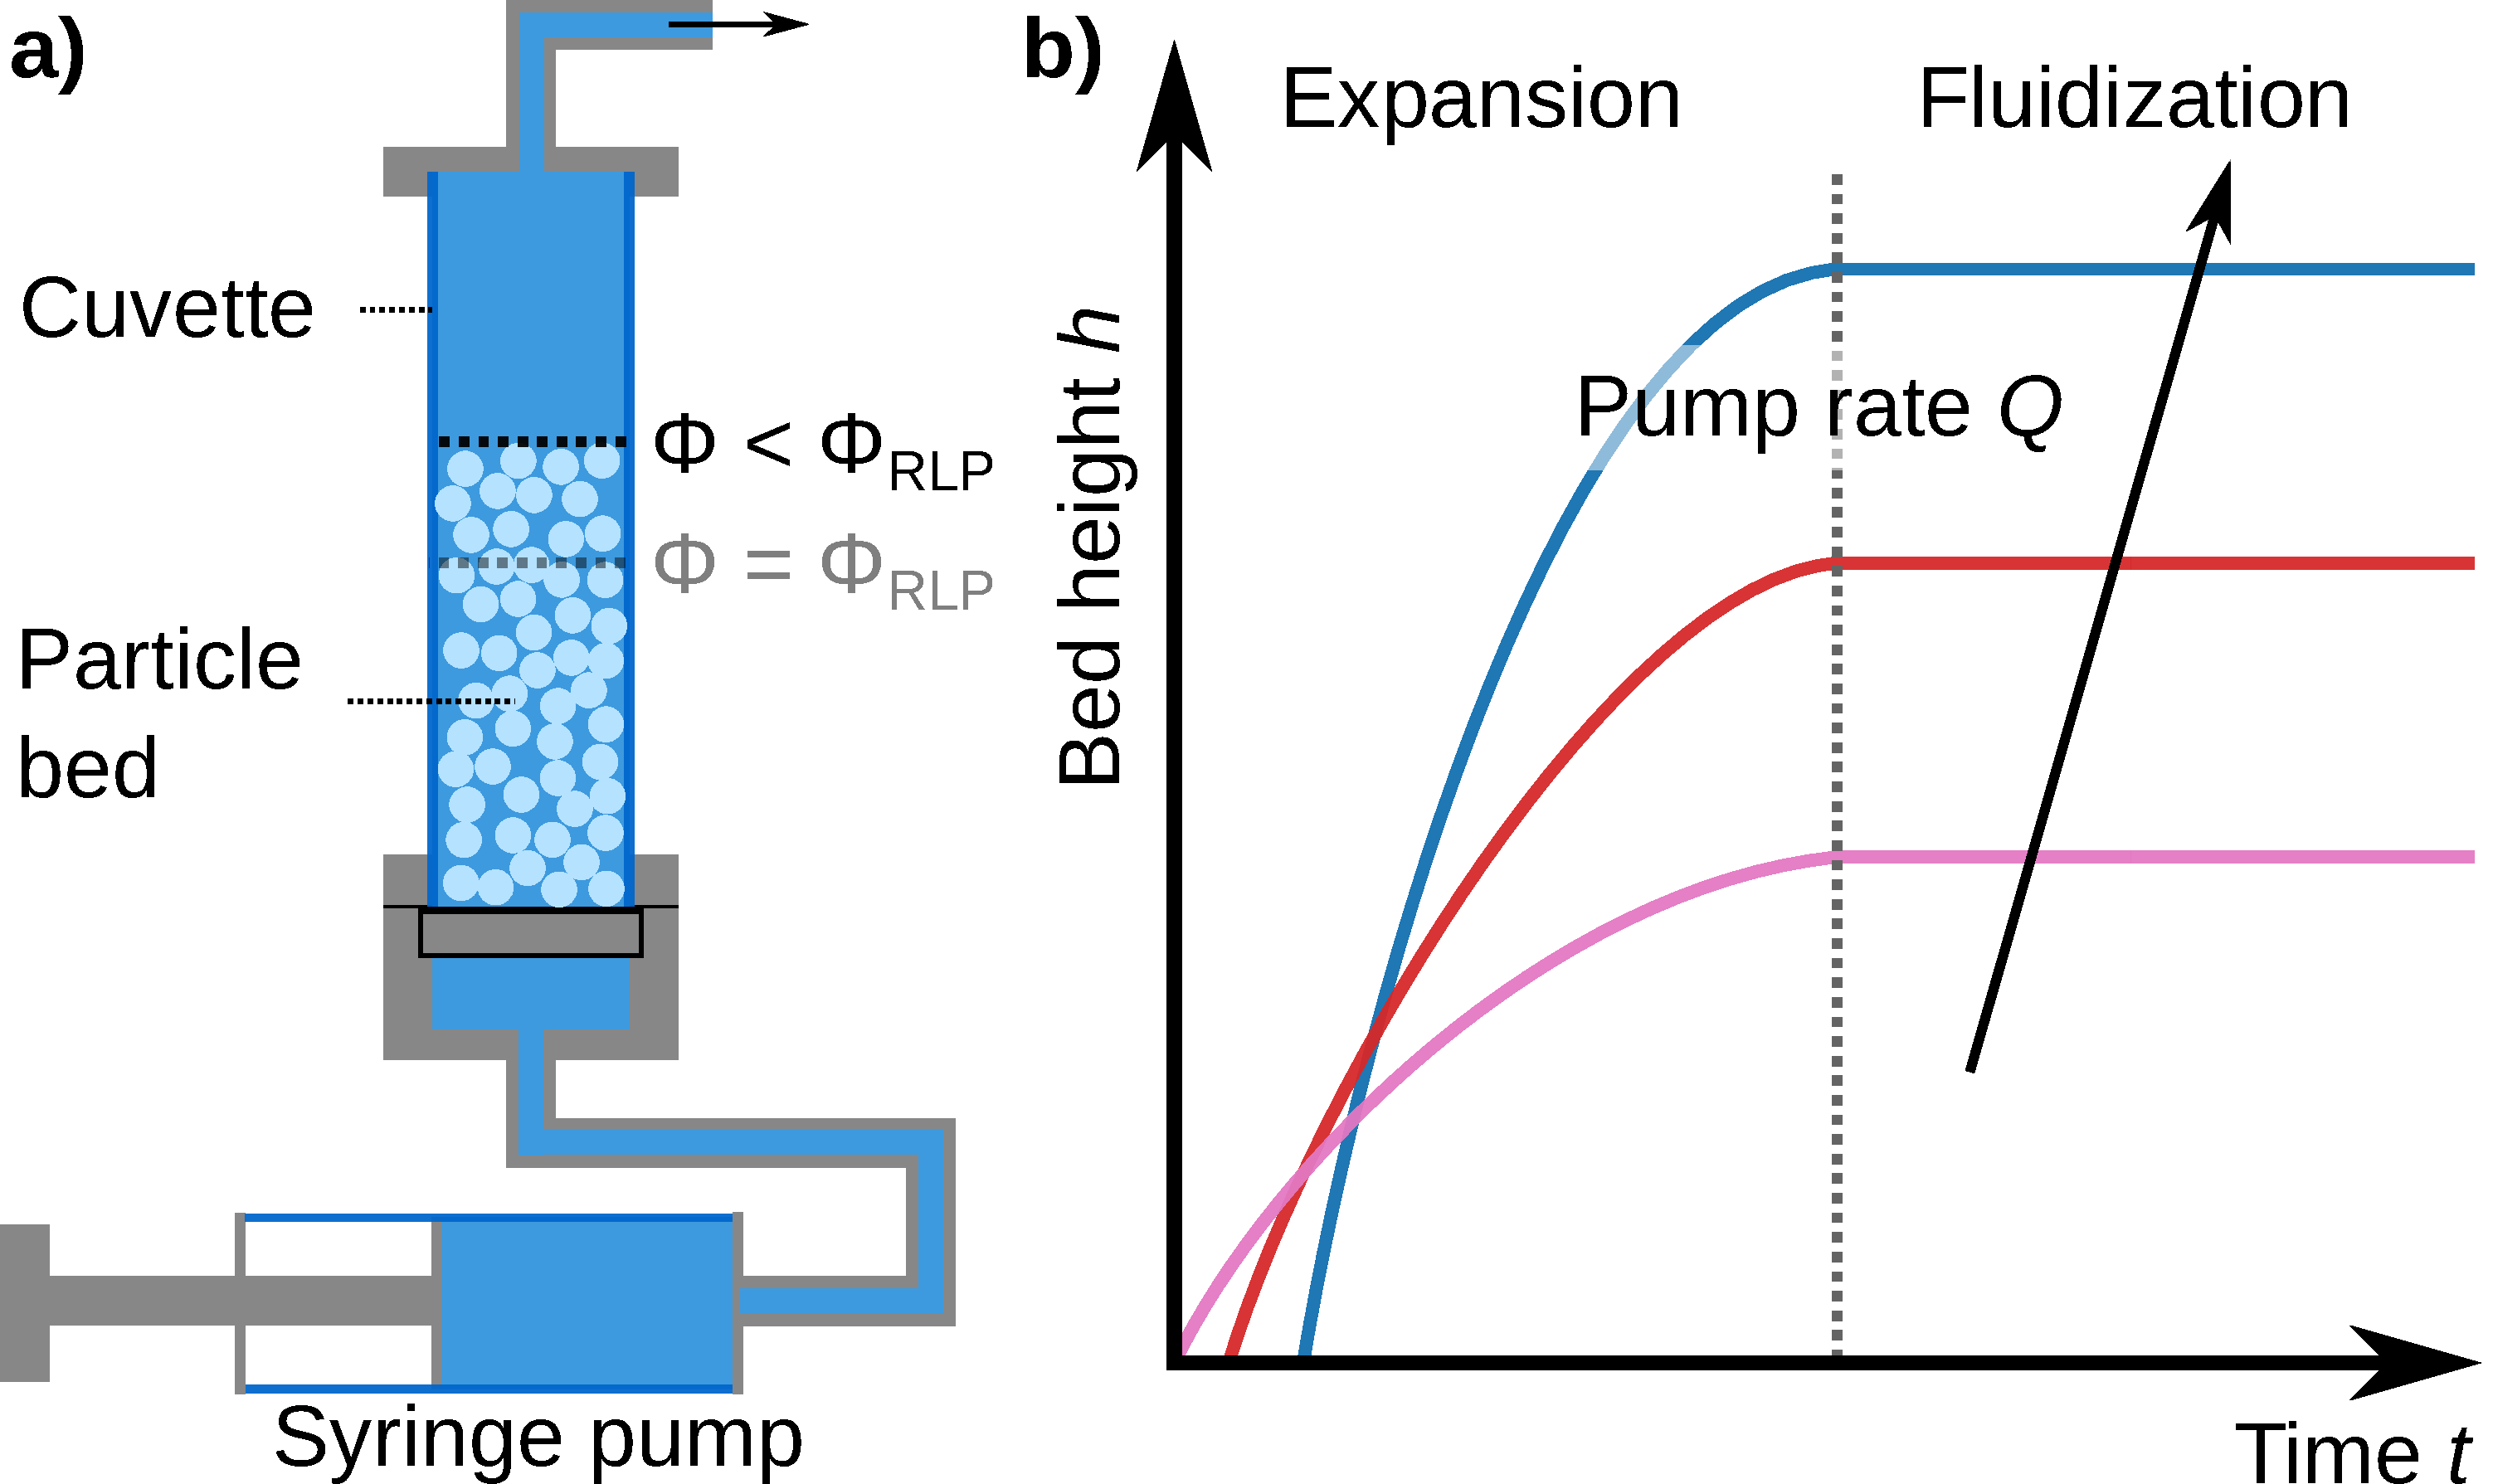
\includegraphics[width=\textwidth]{Sources/motivation/setup-fluidized_bed_final.pdf}}
\end{textblock}

\begin{textblock}{0.5}(0.55,0.1)
	\centering
	\visible<2->{
	\movie[height=0.75\textheight,loop]
	{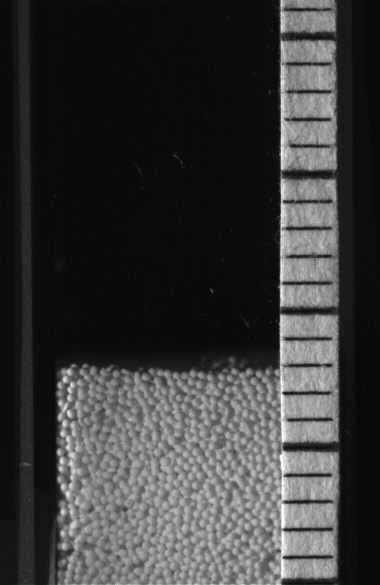
\includegraphics[height=0.75\textheight]{Sources/motivation/video_welm_paetzold.png}}	
	{videos/video_welm_paetzold.avi}
	
	{\footnotesize Master thesis Welm Pätzold}\\[0.2
	cm]
	
	\textcolor{red}{Particulate flows are \textbf{opaque}}}
\end{textblock}
}



%% X-RAY RADIOGRAPHY
\frame{
\begin{tikzpicture}[remember picture,overlay]
\fill[blue1]
(current page.north west) rectangle ([xshift=0.46\paperwidth,yshift=0.33\paperheight]current page.west|-{pic cs:end});
\end{tikzpicture}

\begin{textblock}{0.5}(0.02,0.03)
	\textcolor{white}{
		\Large X-ray radiography \& tomography}
\end{textblock}

\begin{textblock}{0.7}(0.02,0.05)
	\centering
	\only<1>{
	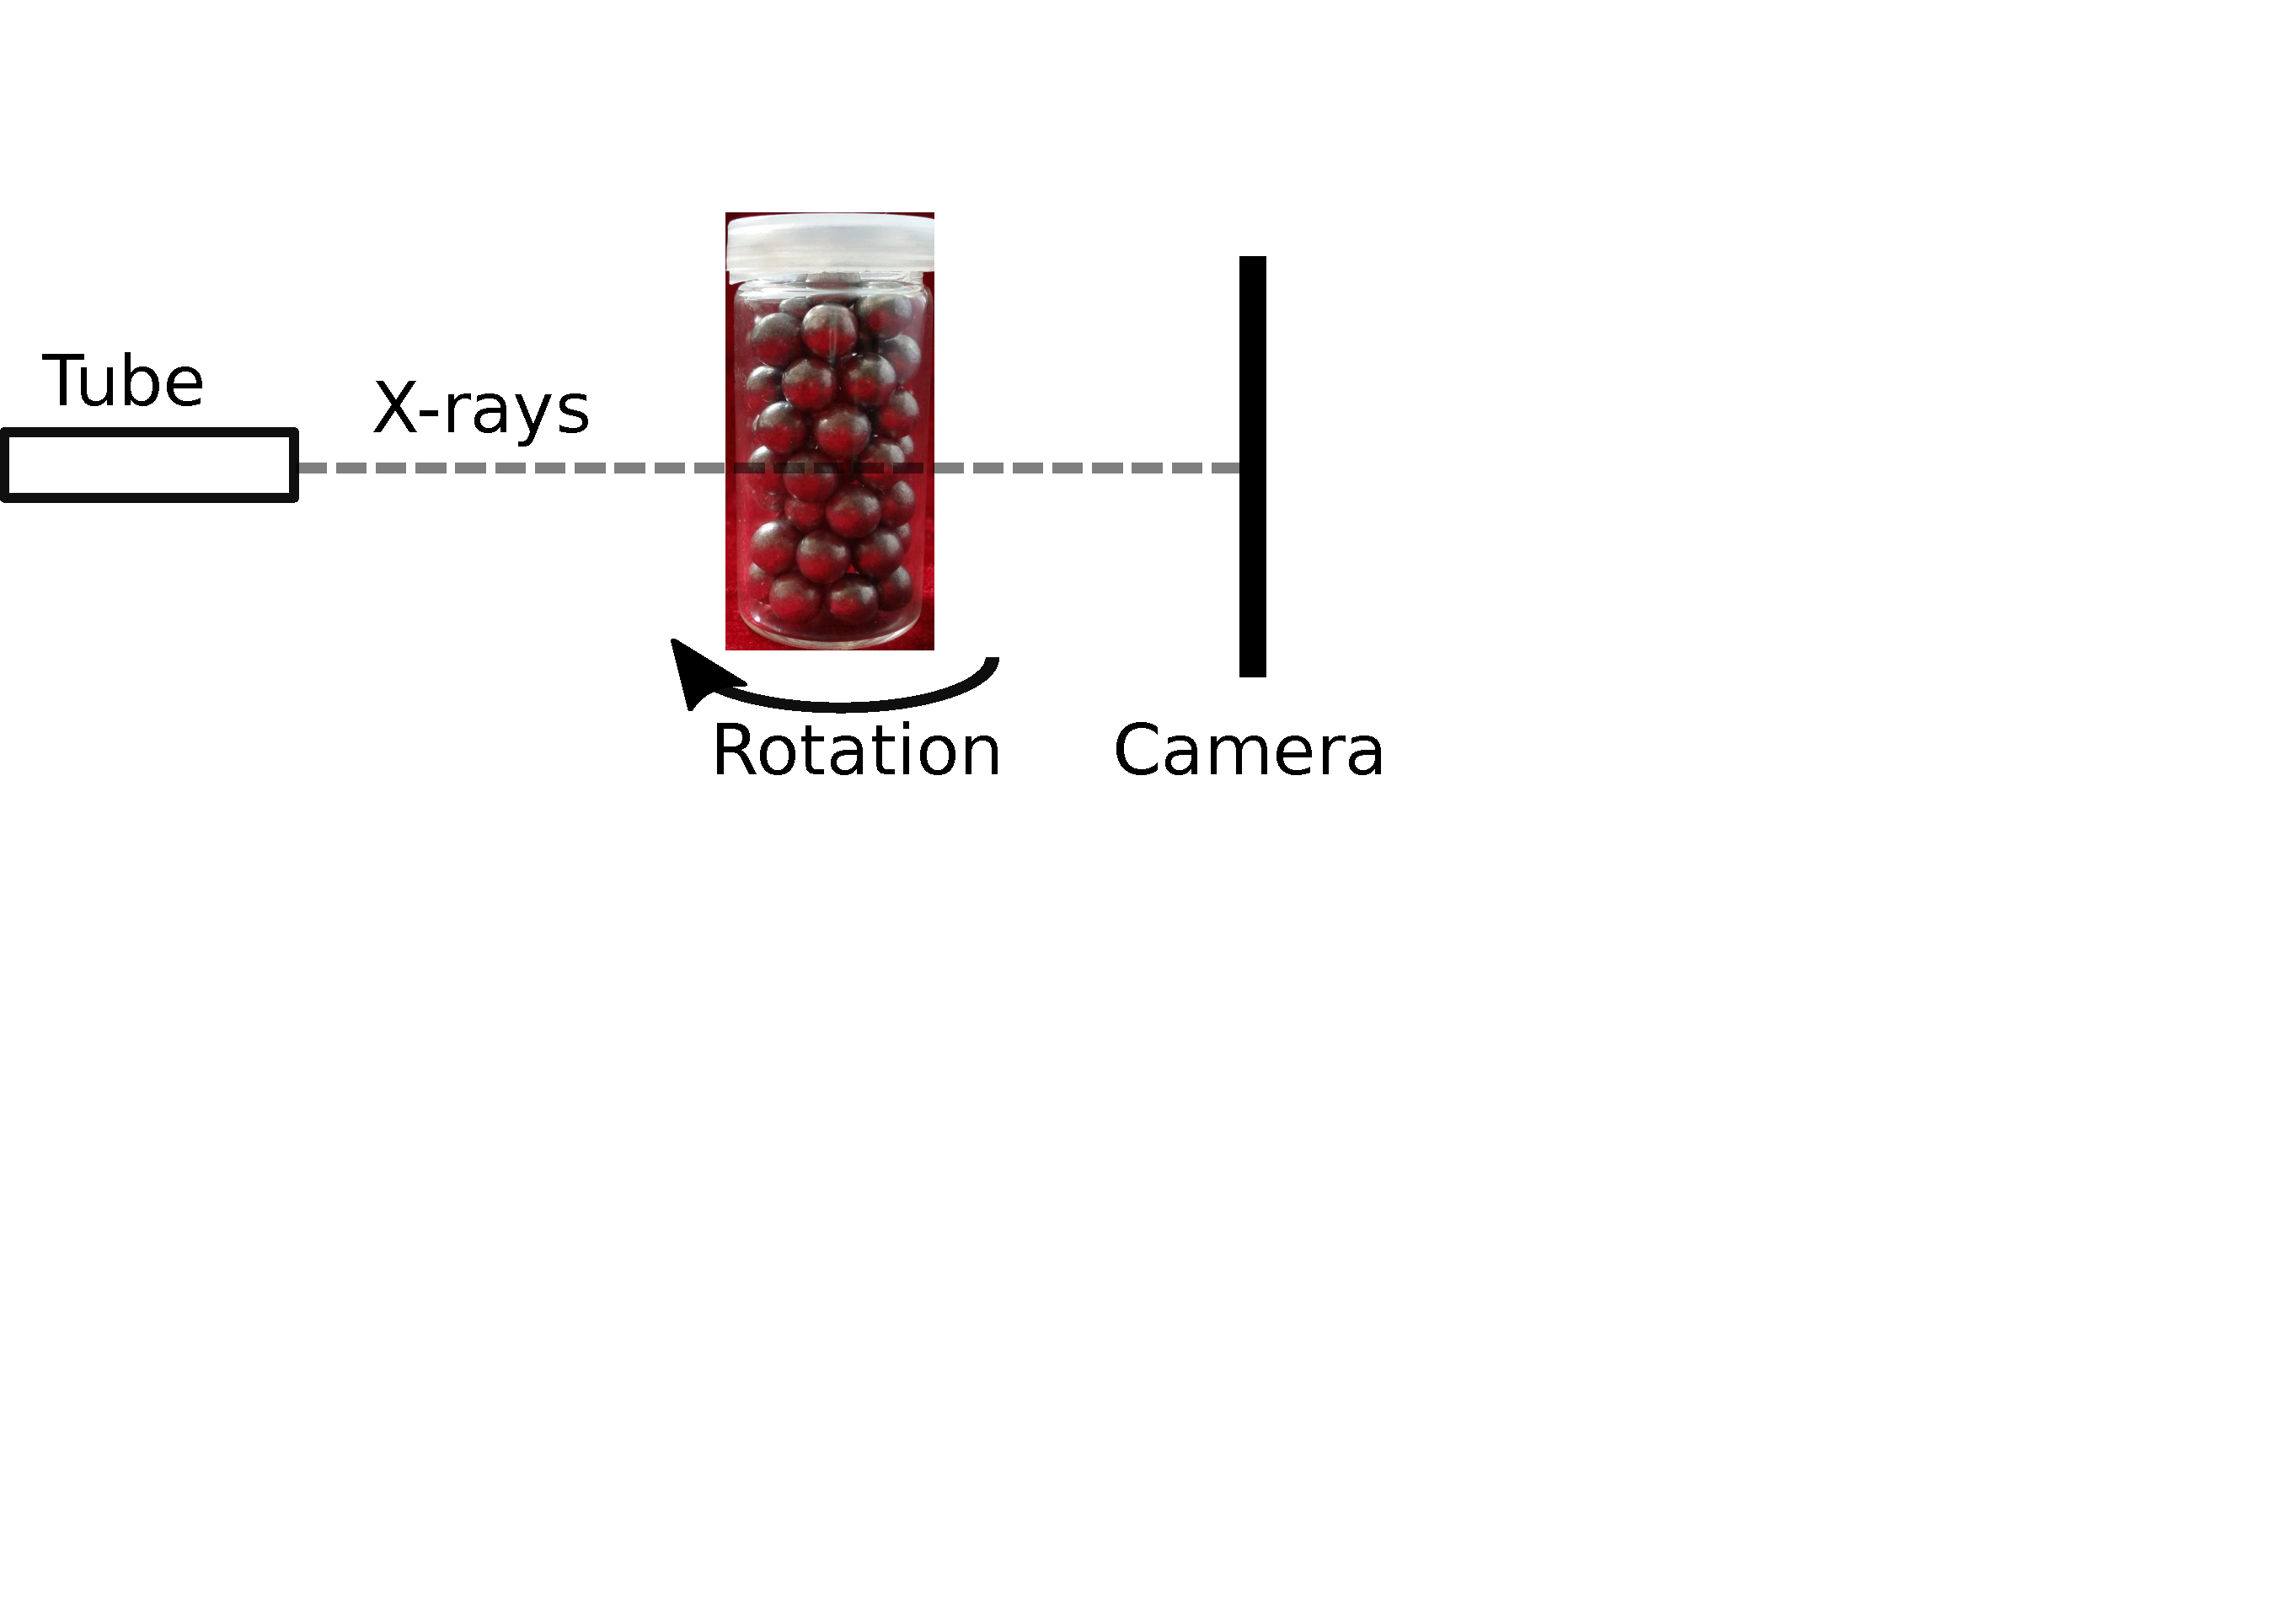
\includegraphics[width=\textwidth]{Sources/motivation/x-ray_setup_use0.pdf}}
	\visible<2->{
	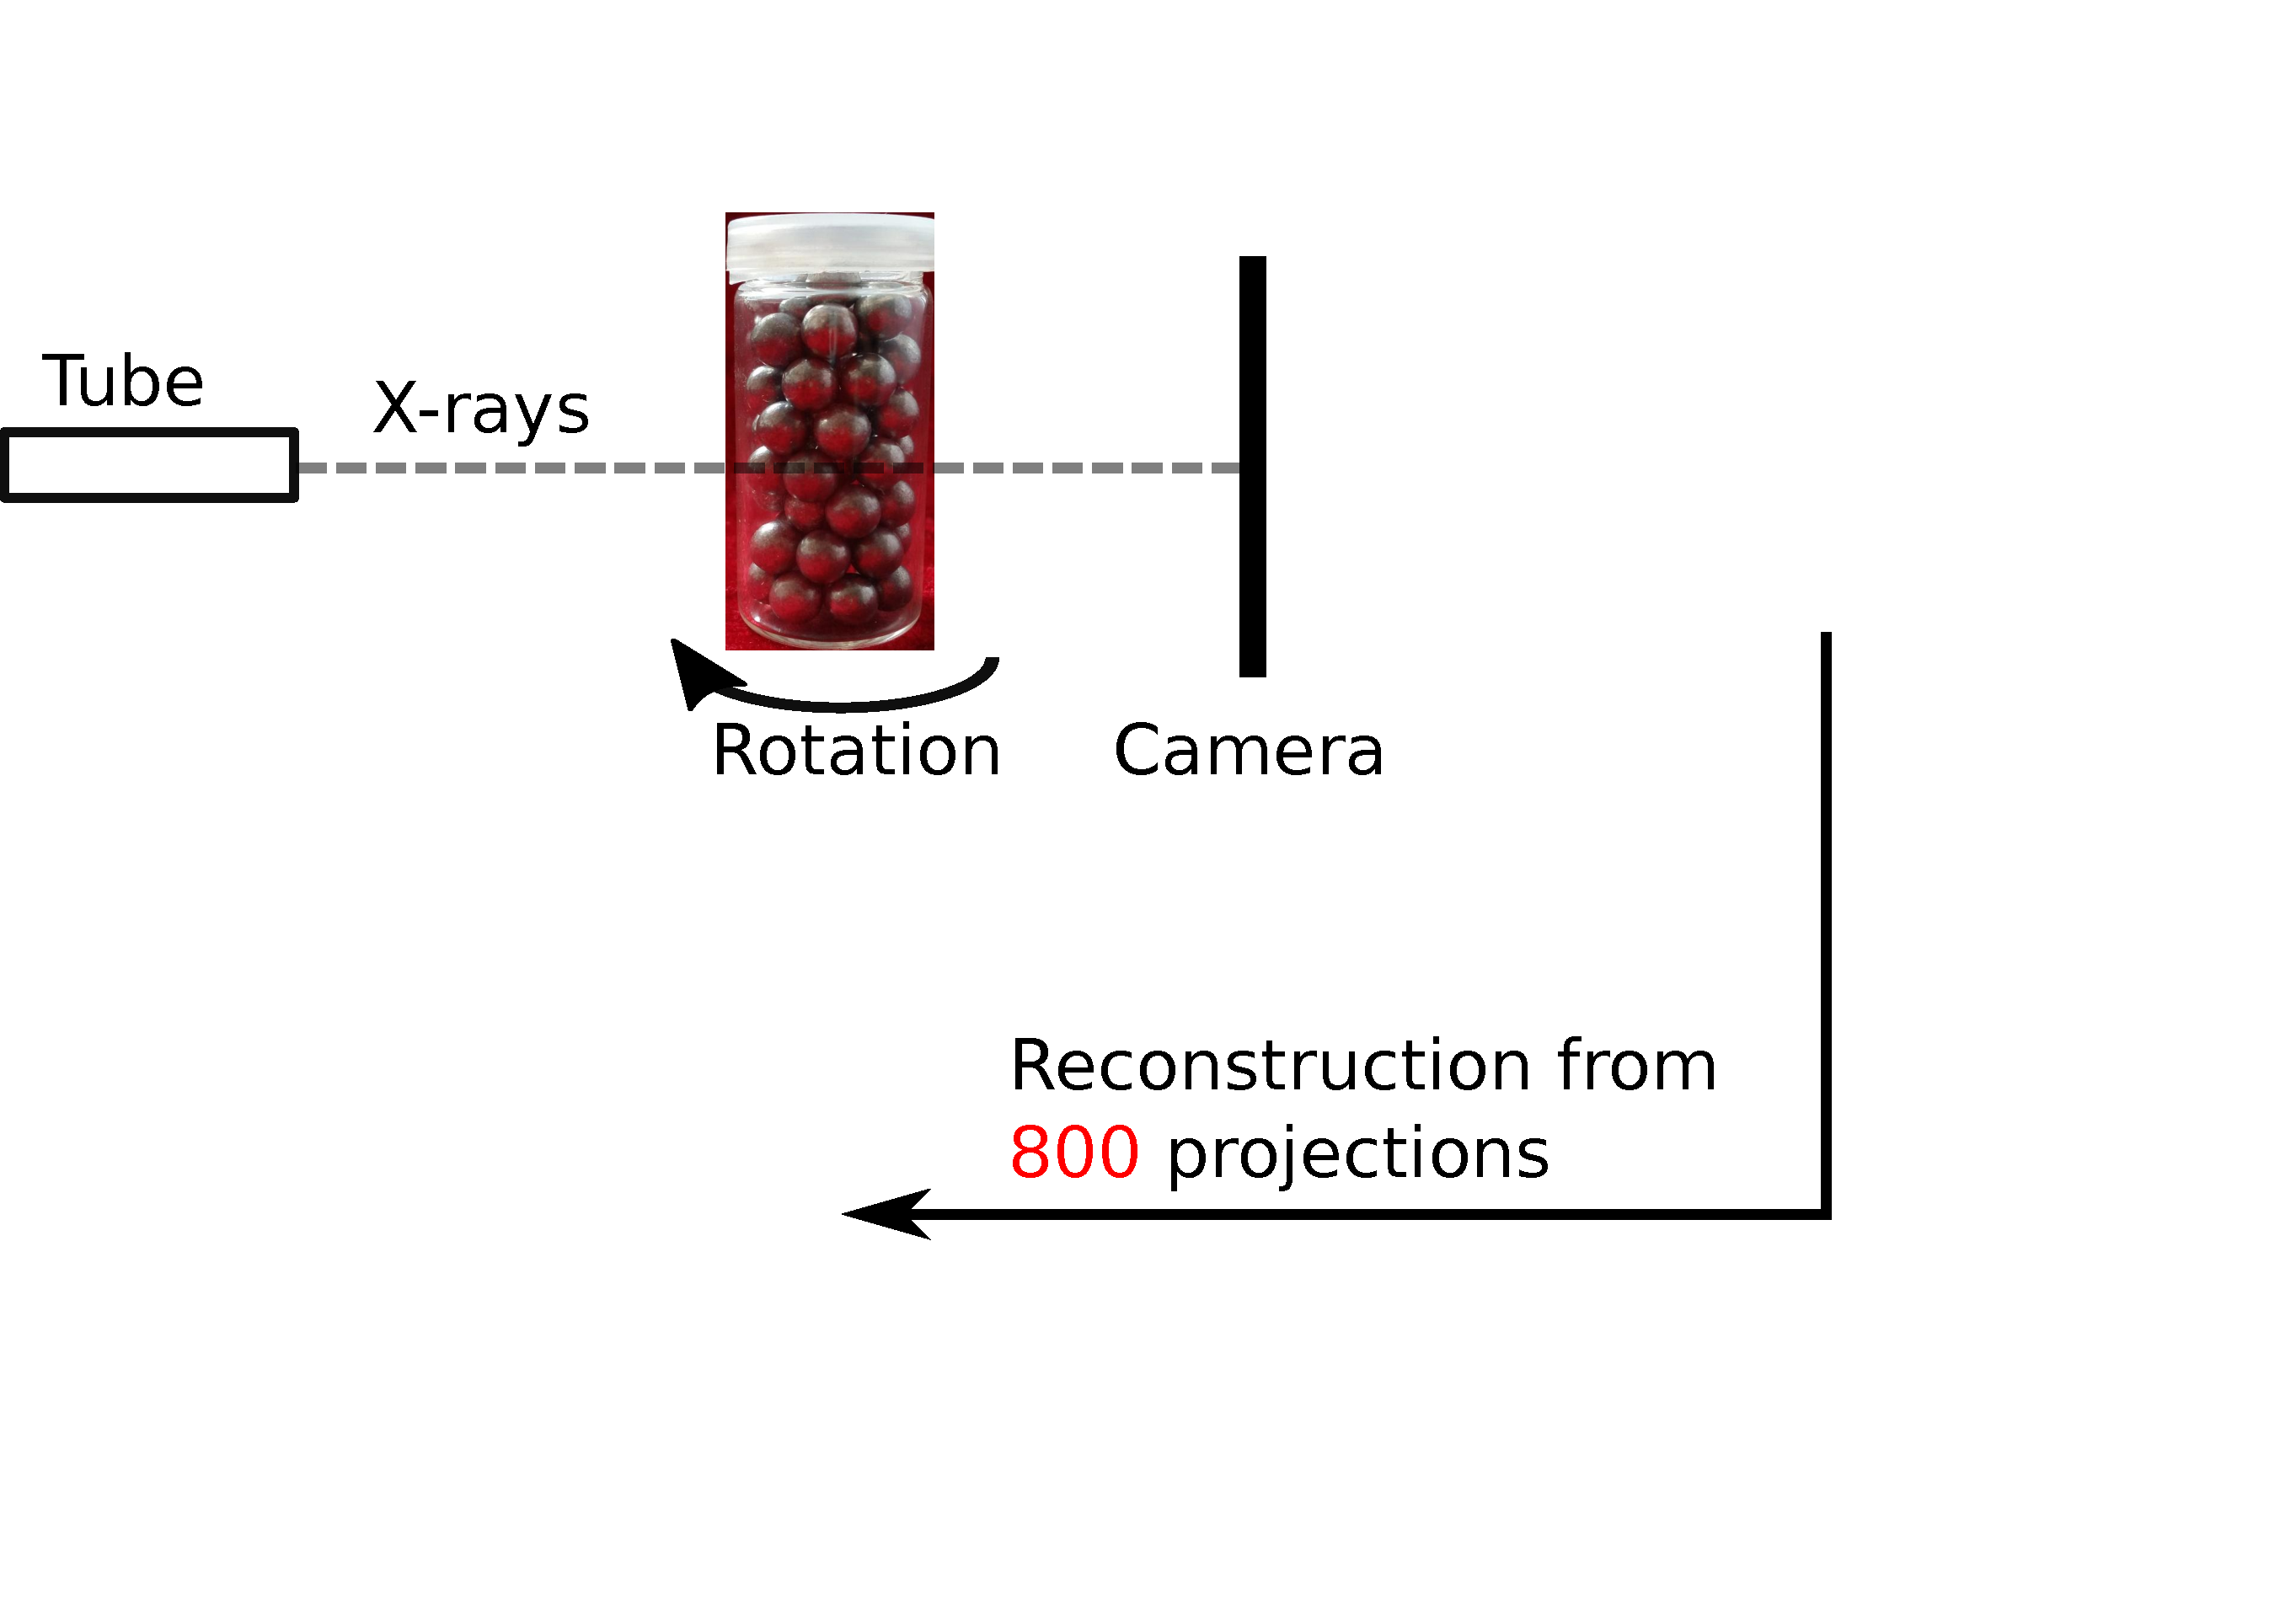
\includegraphics[width=\textwidth]{Sources/motivation/x-ray_setup_use.pdf}}
\end{textblock}

%% Video of Projections
\begin{textblock}{0.22}(0.45,0.06)
	\visible<1->{
	\centering
	Radiogram\\
	\fbox{\parbox{\textwidth}{
	\movie[width =\textwidth,loop]
	{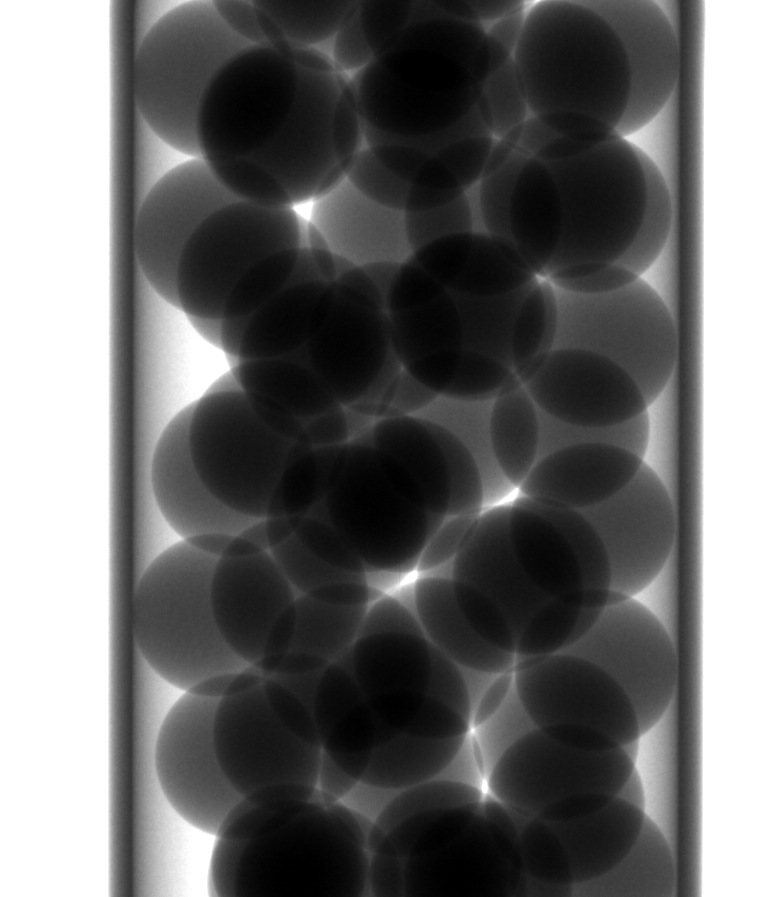
\includegraphics[width=\textwidth]{Sources/motivation/Projection0000.png}}
	{videos/Projections360degree.avi}}}}
\end{textblock}

\begin{textblock}{0.28}(0.7,0.25)
	\visible<1->{
	2D projections of 3D object\\
	\textcolor{blue1}{Short} acquisition time}\\
	$\rightarrow$ \textcolor{blue1}{Dynamic} system
\end{textblock}

% Video of Tomography
\begin{textblock}{0.2}(0.05,0.48)
	\visible<2->{
	\centering
	Tomogram\\
	\movie[width =\textwidth,loop]
	{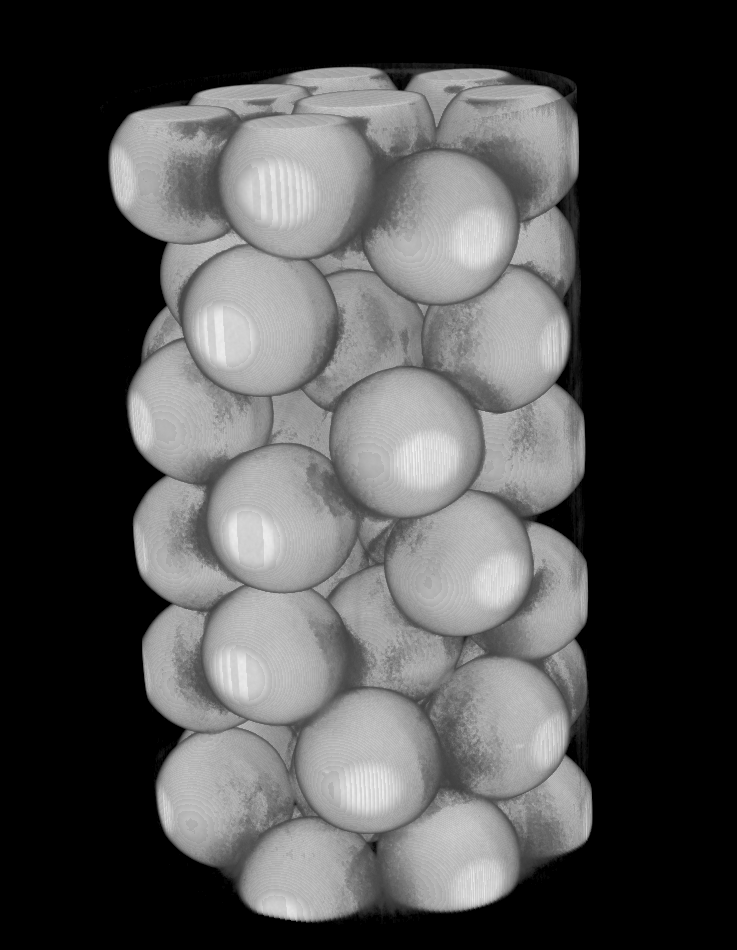
\includegraphics[width=\textwidth]{Sources/motivation/Images_tomo_movie0000.png}}
	{videos/tomogram_360degree.avi}}
\end{textblock}

\begin{textblock}{0.5}(0.27,0.8)
	\visible<2->{
	Full 3D information\\
	\textcolor{red}{Long} acquisition time\\
	$\rightarrow$ \textcolor{red}{Static} objects}
\end{textblock}
}


